
%(BEGIN_QUESTION)
% Copyright 2006, Tony R. Kuphaldt, released under the Creative Commons Attribution License (v 1.0)
% This means you may do almost anything with this work of mine, so long as you give me proper credit

Electrical signals are frequently used in industrial control applications to communicate information from one device to another.  An example of this is motor speed control, where a computer outputs a speed command signal to a motor ``drive'' circuit, which then provides metered power to an electric motor:

$$\includegraphics[width=15.5cm]{i00128x01.eps}$$

Two common standards for analog control signals are 1-5 volts DC and 4-20 mA DC.  In either case, the motor will spin faster when this signal from the computer grows in magnitude (1 volt = motor stopped, 5 volts = motor runs at full speed; or 4 mA = motor stopped, 20 mA = motor runs at full speed).

At first, it would seem as though the choice between 1-5 volts and 4-20 mA as control signal standards is arbitrary.  However, one of these standards exhibits much greater immunity to induced noise along the two-wire cable than the other.  Shown here are two equivalent schematics for these signal standards, complete with an AC voltage source in series to represent the ``noise'' voltage picked up along the cable's length:

$$\includegraphics[width=15.5cm]{i00128x02.eps}$$

Use the Superposition theorem to qualitatively determine which signal standard drops the greatest amount of noise voltage across the motor drive input's resistance, thereby most affecting the motor speed control.

\underbar{file i00128}
%(END_QUESTION)





%(BEGIN_ANSWER)

The motor drive input in the 1-5 volt signal system ``sees'' more noise voltage than the motor drive input in the 4-20 mA signal system.

\vskip 10pt

Follow-up question: what bad effects do you think noise superimposed on the DC signal cable would have on motor speed control?

\vskip 10pt

Challenge question: why do you suppose the 1-5 volt signal system requires a much greater input impedance (1 M$\Omega$) than the 4-20 mA signal system?  What might happen to the voltage signal received at the motor drive's input terminals if the input resistance were much less?

%(END_ANSWER)





%(BEGIN_NOTES)

This is a very practical question, as induced noise is no academic matter in real industrial control systems.  This is especially true around motor drive circuits, which are well known for their ability to generate {\it lots} of electrical noise!

Some students may suggest that the distinction between voltage and current signals is moot because shielded-pair cable is suppose to all but eliminate induced noise.  In answer to this (good) question, it should be noted that real-life conditions are never ideal, and that induced noise (to some degree) is an unavoidable fact of life, especially in many industrial environments.

The challenge question may seem unanswerable until one considers the unavoidable resistance along the length of the signal cable and calculates the effects of voltage drop along the wire length for a huge input resistance versus a small input resistance.

%INDEX% Basics, instrumentation signals: 1-5 V versus 4-20 mA signals
%INDEX% Basics, instrumentation signals: signal noise immunity

%(END_NOTES)


